% !TeX spellcheck = ru_RU
% !TEX root = vkr.tex

\section{Общая архитектура решения}

\subsection{Реализация модуля с топологией RNN GRU}
\label{subsec:topology}


Основная идея данного модуля --- предоставить возможность создания GRU-сети в рамках существующей архитектуры \texttt{DEGANN}. Для этого был разработан класс \texttt{TensorflowGRUNet}, который наследуется от \texttt{tf.keras.Model}\cite{tensorflowDoc} и определяет необходимую логику построения слоёв GRU, их инициализацию, а также способ компоновки выходных данных. Важным моментом является то, что реализация идёт в связке с существующей инфраструктурой \texttt{DEGANN}, где выбор конкретной топологии сети (в данном случае GRU) осуществляется через параметр \texttt{net\_type}, передаваемый при создании экземпляра класса \texttt{IModel}.

\subsubsection{Основные параметры и их назначение}
Класс \texttt{TensorflowGRUNet} включает несколько важных параметров, которые определяют архитектуру сети:
\begin{itemize}
    \item \textbf{input\_size:} размер входных данных. Задаёт количество входных признаков в данных.
    \item \textbf{block\_size:} список, определяющий количество нейронов в каждом слое GRU. Все слои должны иметь одинаковое количество нейронов.
    \item \textbf{output\_size:} количество выходных нейронов. Обычно для задач регрессии используется один выходной нейрон.
    \item \textbf{activation\_func и recurrent\_activation:} функции активации для основного состояния и рекуррентного состояния соответственно. По умолчанию используются \texttt{tanh} и \texttt{sigmoid}, так как они являются стандартными для GRU.
    \item \textbf{dropout\_rate:} уровень dropout, добавляемый после каждого слоя GRU для предотвращения переобучения.
    \item \textbf{weight и biases:} инициализаторы весов и смещений. Используются случайные значения в заданном диапазоне для начальной настройки параметров модели.
    \item \textbf{return\_sequences:} флаг, определяющий, будет ли сеть возвращать последовательности — это важно для многослойных рекуррентных сетей.
\end{itemize}

Данные параметры позволяют гибко настраивать модель под задачу, сохраняя при этом целостность и удобство использования в экосистеме \texttt{DEGANN}.

\subsubsection{Интеграция в \texttt{DEGANN}:}
Для внедрения новой архитектуры в \texttt{DEGANN} мы используем существующий интерфейс \texttt{IModel}. Создание модели осуществляется примерно следующим образом: при инициализации \texttt{IModel} мы передаем параметр \texttt{net\_type="GRUNet"}, что приводит к созданию внутри экземпляра класса сети с топологией \texttt{TensorflowGRUNet}.

Создание модели с топологией GRU происходит следующим образом:

\begin{lstlisting}[language=Python, caption=Создание модели с использованием топологии GRUNet, numbers=left]
count_size = 5  # количество слоёв
gru_units = 30  # количество нейронов в слое
shape = [gru_units] * count_size
GRU_IModel = IModel(
    input_size=1,
    output_size=1,
    net_type="GRUNet",  # топология GRUNet
    block_size=shape)   # передаём размеры слоёв
\end{lstlisting}

В данном случае, внутри класса \texttt{IModel} вызывается метод \texttt{\_create\_functions["GRUNet"]}, возвращающий экземпляр \texttt{TensorflowGRUNet}, унаследованный от \texttt{tf.keras.Model}. Таким образом, мы сохраняем единообразный интерфейс для работы с моделями различных типов (DenseNet, GRUNet и т.д.) внутри \texttt{DEGANN}.

\subsubsection{Как работает класс TensorflowGRUNet}
При инициализации класс \texttt{TensorflowGRUNet} создаёт несколько GRU-слоёв, каждый из которых имеет одинаковое количество нейронов, заданное параметром \texttt{block\_size}. На этапе инициализации происходит проверка, чтобы все слои сети имели одинаковый размер, поскольку это важное условие для корректной работы рекуррентных нейронных сетей. Если размер слоёв отличается, выбрасывается исключение.

После каждого GRU-слоя добавляется слой Dropout для предотвращения переобучения. Эти слои помогают повысить устойчивость модели, добавляя случайные обнуления нейронов во время тренировки.

\subsubsection{Реализация функции call}
Функция \texttt{call} является важной частью класса \texttt{TensorflowGRUNet}, поскольку она выполняет прямой проход через сеть. В этой функции данные проходят через все GRU-слои, а затем через выходной полносвязный слой, который выполняет линейную активацию для задач регрессии.

\subsubsection{Особенности реализации}
Ключевой особенностью реализации является соблюдение совместимости с другими компонентами библиотеки DEGANN, что позволяет использовать стандартные методы обучения, тестирования и экспорта моделей. Например, параметры модели могут быть экспортированы в виде словаря, что упрощает сохранение и интеграцию в другие модули. Метод \texttt{to_dict} позволяет сохранить ключевые параметры модели, такие как тип сети, количество нейронов в слоях, количество слоёв и выходной размер, в виде словаря для дальнейшего использования или интеграции с другими частями системы.




\subsection{Создание модели и реализация callback-функций}
\label{subsec:model_callbacks}

\subsubsection{Создание модели GRU}
Для создания модели с использованием топологии GRU использовалась модульная архитектура DEGANN, наследуемую от базового класса \texttt{IModel}, не внося изменений в его структуру. Такой подход позволил адаптировать сеть GRU к задачам аппроксимации дифференциальных уравнений и интегрировать её в существующий функционал проекта.

\subsubsection{callbacks}
В процессе разработки и обучения модели важно не только корректно настроить её архитектуру, но и обеспечить инструментами, позволяющими наглядно оценивать ход обучения, качество модели и её производительность. Это включает как отслеживание ключевых метрик, таких как функция потерь, так и визуализацию предсказаний модели на различных этапах.

Основные цели анализа обучения и валидации включают:
\begin{itemize}
    \item \textbf{Оценка функции потерь}: Анализ функции потерь на тренировочных и валидационных данных позволяет выявить динамику обучения, а также возможные проблемы, такие как переобучение или недостаточное обучение.
    \item \textbf{Раннее прекращение обучения}: Обеспечивает остановку обучения, если модель перестала улучшаться, предотвращая ненужные вычисления и переобучение.
    \item \textbf{Сохранение лучшей модели}: Позволяет фиксировать параметры модели с минимальной валидационной ошибкой, чтобы использовать её для дальнейших экспериментов.
    \item \textbf{Визуализация}: Сравнение предсказаний модели с истинной функцией и визуализация потерь предоставляет интуитивное понимание, насколько хорошо модель аппроксимирует данные.
    \item \textbf{Измерение времени обучения}: Позволяет оценить, насколько эффективно используются вычислительные ресурсы при обучении модели.
\end{itemize}

Для достижения этих целей были реализованы и интегрированы несколько callback-функций, обеспечивающих автоматическое выполнение перечисленных выше задач. Эти callback-функции разработаны как часть архитектуры проекта DEGANN и могут быть легко добавлены при обучении любой модели.


\subsubsection{Пример использования callback-функций}

Для анализа и визуализации обучения были разработаны и внедрены следующие callback-классы:
\begin{itemize}
    \item \texttt{LossTracking}: Отслеживает и сохраняет значения функции потерь на тренировочных и валидационных данных.
    \item \texttt{EarlyStopping}: Реализует раннее прекращение обучения при отсутствии улучшений в течение заданного количества эпох.
    \item \texttt{SaveBestModel}: Сохраняет параметры модели с минимальной валидационной ошибкой.
    \item \texttt{VisualizationTS}: Визуализирует процесс обучения и предсказания модели, сравнивая их с истинной функцией.
\end{itemize}

Ниже приведён пример использования данных callback-функций в процессе обучения модели GRU:

\begin{lstlisting}[language=Python, breaklines, caption=Пример настройки и использования callback-функций, numbers=left]
from degann.networks.callbacks import MeasureTrainTime, LossTracking, EarlyStopping, SaveBestModel, VisualizationTS

MeasureTrainTime = MeasureTrainTime()
Loss_tracking = LossTracking()
Early_stopping = EarlyStopping(patience=100)  # "patience" - the number of epochs without improvement
Save_best_model = SaveBestModel(GRU_IModel)
Visualization = VisualizationTS(train_data_x, train_data_y, val_data_x, val_data_y, name_dataset.split('_')[0], funcs)

GRU_IModel.train(train_data_x, train_data_y, validation_data=(val_data_x, val_data_y), epochs=epochs, verbose=0, callbacks=[MeasureTrainTime, Loss_tracking, Early_stopping, Save_best_model, Visualization])
\end{lstlisting}

\begin{lstlisting}[language=Tex, breaklines, caption=Пример получения данных от callback-функций]
Epoch 1: finished in: 6.68 seconds | Training Loss: 0.4940, Validation Loss: 0.4203
Epoch 2: finished in: 0.97 seconds | Training Loss: 0.4340, Validation Loss: 0.4031
Epoch 3: finished in: 1.05 seconds | Training Loss: 0.3875, Validation Loss: 0.3818
Epoch 4: finished in: 1.08 seconds | Training Loss: 0.3203, Validation Loss: 0.2576
Epoch 5: finished in: 1.09 seconds | Training Loss: 0.2171, Validation Loss: 0.1123
...
Epoch 49: finished in: 0.40 seconds | Training Loss: 0.0597, Validation Loss: 0.0272
Epoch 50: finished in: 0.48 seconds | Training Loss: 0.0617, Validation Loss: 0.0411
Total training time: 55.3523 seconds
Average time per epoch: 1.107045 seconds
Loss before training = 0.606187
Loss after training = 0.059869
different between Losses =0.546318
validation loss before training = 0.610131
validation loss after training = 0.041137
Difference in validation loss = 0.568993
\end{lstlisting}

\subsubsection{Описание callback-функций}

\textbf{LossTracking}: Позволяет отслеживать значения функции потерь на тренировочных и валидационных данных на каждой эпохе.

\textbf{EarlyStopping}: Реализует механизм ранней остановки обучения, если валидационная ошибка не уменьшается в течение заданного числа эпох \textbf{patience}. Это помогает избежать переобучения и экономит ресурсы.

\textbf{SaveBestModel}: Сохраняет лучшую модель, найденную в процессе обучения, фиксируя параметры сети с минимальной валидационной ошибкой.

\textbf{VisualizationTS}: Генерирует графики, отображающие:
\begin{itemize}
    \item Динамику функции потерь на тренировочных и валидационных данных.
    \item Сравнение истинной функции, предсказаний модели и тренировочных данных.
\end{itemize}

Данные callback-функции позволяют автоматизировать рутинные задачи анализа и визуализации обучения, делая процесс более удобным и наглядным.




\section{Валидация решения}



\subsection{Датасет и сложно-аппроксимируемая функция}
\label{subsec:dataset}

\subsubsection{Генерация датасета}
Для тестирования работы архитектуры GRU-сети был подготовлен специальный датасет, который генерировался с помощью встроенных инструментов библиотеки \texttt{DEGANN}. В качестве сложно-аппроксимируемой функции была выбрана функция \texttt{hardsin}, которая была добавлена в модуль \texttt{functions.py}:

Эта функция обладает сложной математической структурой, что делает её трудно аппроксимируемой стандартными архитектурами нейронных сетей. Её аналитическое выражение имеет следующий вид:

\[
f(x) = \sin\left(\ln(x^{\sin(10x)})\right)
\]

\subsubsection{График функции}
На рисунке ниже представлен график функции \texttt{hardsin}, демонстрирующий её сложное поведение:

\begin{figure}[H]
    \centering
    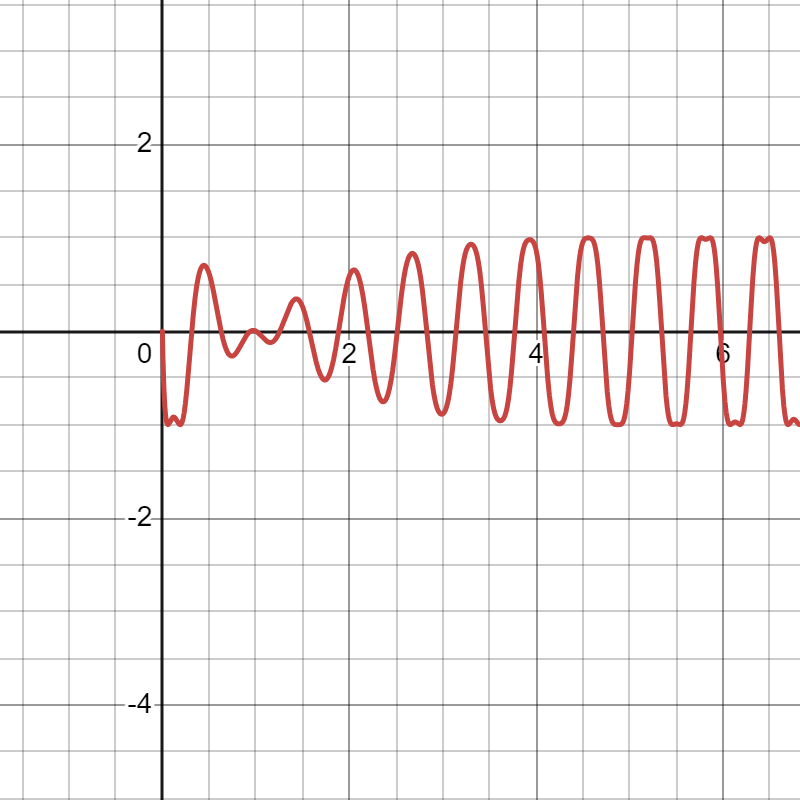
\includegraphics[width=0.5\textwidth]{figures/graph_hardsin.png}
    \caption{График функции $f(x) = \sin\left(\ln(x^{\sin(10x)})\right)$}
    \label{fig:hardsin_graph}
\end{figure}

\subsubsection{Добавление шума}

Для повышения устойчивости модели и её способности к обобщению в процессе обучения на тренировочные данные добавлялся шум, который следовал нормальному распределению. Это позволяет модели лучше адаптироваться к реальным данным, которые часто содержат случайные колебания и погрешности. Нормальное распределение (также называемое гауссовским распределением) является одним из наиболее часто используемых видов распределений в статистике и машинном обучении.

\paragraph{Формула нормального распределения:}
Нормальное распределение определяется следующей плотностью вероятности:

\[
f(x) = \frac{1}{\sqrt{2 \pi \sigma^2}} e^{-\frac{(x - \mu)^2}{2 \sigma^2}}
\]

где:
\begin{itemize}
    \item $\mu$ - математическое ожидание (среднее значение),
    \item $\sigma$ - стандартное отклонение (мера разброса данных),
    \item $x$ - случайная величина.
\end{itemize}

Параметры $\mu$ и $\sigma$ в нашем случае были рассчитаны на основе целевой переменной тренировочного датасета $\texttt{train\_data\_y}$, чтобы шум соответствовал масштабу данных.

\paragraph{Применение шума в датасете:}
Добавление шума выполнялось с использованием библиотеки NumPy, где функция \texttt{np.random.normal()} генерирует массив случайных значений, следующих нормальному распределению. В нашем случае среднее значение шума $\mu = 0$, а стандартное отклонение рассчитывается как $0.1 \cdot \sigma$, где $\sigma$ --- стандартное отклонение значений целевой переменной. Формула добавления шума выглядит следующим образом:

\[
\texttt{train\_data\_y\_noisy} = \texttt{train\_data\_y} + \xi, \quad \xi \sim \mathcal{N}(0, 0.1 \cdot \sigma)
\]

\subsubsection{Загрузка и обработка данных}
Для создания тренировочного и валидационного наборов данных использовались встроенные методы генерации датасетов в \texttt{DEGANN}, которые позволяют сохранять данные в формате \texttt{.csv} для последующего использования.


\subsubsection{Временные последовательности}
Рекуррентные нейронные сети, такие как GRU, предназначены для обработки временных последовательностей. Их ключевая особенность заключается в возможности сохранять информацию о предыдущих состояниях для анализа текущих данных. Это делает их идеальными для задач, где данные зависят от контекста, например, аппроксимация временных рядов.

Для корректной работы RNN данные из исходного датасета были преобразованы в последовательности фиксированной длины с помощью функции \texttt{create sequences}:

\begin{lstlisting}[language=Python, breaklines, caption=Создание временных последовательностей,numbers=left]
def create_sequences(data_x, data_y, time_steps):
    x, y = [], []
    for i in range(len(data_x) - time_steps):
        x.append(data_x[i:i + time_steps])
        y.append(data_y[i + time_steps])
    return np.array(x), np.array(y)

time_steps = 10
train_data_x, train_data_y = create_sequences(train_data_x, train_data_y, time_steps)
val_data_x, val_data_y = create_sequences(val_data_x, val_data_y, time_steps)
\end{lstlisting}

В данном примере \texttt{time\_steps} задаёт количество шагов в последовательности. Это означает, что каждый входной элемент сети состоит из \texttt{time\_steps} предыдущих значений, а целевая переменная соответствует следующему значению функции.

\paragraph{Почему RNN работают с временными последовательностями?}
Основное преимущество RNN заключается в их способности передавать информацию через скрытые состояния (\textit{hidden states}). В отличие от обычных нейронных сетей, которые обрабатывают каждый вход независимо, RNN сохраняют информацию из предыдущих шагов и используют её для обработки текущего ввода. Это реализуется через рекуррентную связь, которая обновляет скрытое состояние на каждом временном шаге.



\subsection{Метрики и настройка гиперпараметров}
\label{subsec:metrics}

Для эффективного обучения моделей на основе архитектуры GRU важен тщательный выбор функции потерь, оптимизатора и гиперпараметров. Этот процесс позволяет достичь баланса между качеством аппрокисмации и вычислительными затратами.

\subsubsection{Функция потерь}

В качестве функции потерь использовалась среднеквадратичная ошибка (\textit{Mean Squared Error}, MSE), определяемая формулой:
\[
\text{MSE} = \frac{1}{n} \sum_{i=1}^{n} (y_i - \hat{y}_i)^2,
\]
где \( y_i \) — истинное значение, \( \hat{y}_i \) — предсказание модели, \( n \) — количество примеров.

Среднеквадратичная ошибка была выбрана по следующим причинам:
\begin{itemize}
    \item MSE минимизирует крупные отклонения между истинными и предсказанными значениями, что особенно полезно при аппроксимации сложных функций.
    \item Эта метрика стандартна для задач регрессии и обеспечивает устойчивую сходимость моделей \cite{Goodfellow}.
\end{itemize}

Таким образом, MSE является подходящим выбором для задач, связанных с аппроксимацией решений дифференциальных уравнений.

\subsubsection{Гиперпараметры модели}

Для данной архитектуры были выбраны параметры, исходя из результатов экспериментов и тестов, при которых наблюдался хороший результат при доступном времени обучения и количестве эпох. Проведённые эксперименты позволили определить следующие параметры:
\begin{itemize}
    \item \textbf{Количество слоёв}: 5;
    \item \textbf{Количество нейронов в каждом слое}: 30.
\end{itemize}

Выбор таких параметров обусловлен следующими факторами:
\begin{itemize}
    \item Увеличение числа слоёв и нейронов значительно повышает сложность модели и требуют большего времени обучения. При этом избыточное увеличение параметров не всегда приводит к заметному улучшению качества, а ограниченные ресурсы накладывают свои ограничения.
    \item Уменьшение количества слоёв или нейронов приводит к недообучению модели, что негативно сказывается на качестве аппроксимации функций.
    \item В выбранной конфигурации модель способна эффективно решать задачи аппроксимации, оставаясь достаточно компактной.
\end{itemize}

\subsubsection{Оптимизатор}

Для оптимизации был выбран \textit{Adam}, поскольку он эффективно регулирует скорость обучения для каждого параметра и демонстрирует высокую стабильность в задачах регрессии \cite{HOML}. \textit{Adam} сочетает преимущества методов \textit{Momentum} и \textit{RMSprop}, что делает его особенно полезным при обучении рекуррентных сетей, таких как GRU.

Преимущества выбора оптимизатора \textit{Adam}:
\begin{itemize}
    \item Автоматическая адаптация шага обучения для быстрого достижения сходимости.
    \item Хорошие результаты при обучении моделей, работающих с временными последовательностями \cite{adam}.
    \item Стабильность градиентного спуска, что особенно важно для задач с длительными зависимостями.
\end{itemize}

Таким образом, выбор MSE в качестве функции потерь, использование оптимизатора \textit{Adam} и разумная конфигурация гиперпараметров обеспечивают эффективное обучение модели. Данная настройка параметров позволяет достичь приемлемого качества аппроксимации функций в условиях ограниченных вычислительных ресурсов.
